% =====================================================================
% Marco Práctico --- Sección 3.6: Fase 1
% =====================================================================

\subsection{Etapa 1 --- Núcleo del Dispositivo Memristivo y Variabilidad}
\label{ch:fase1}

Esta sección describe la implementación y simulación de modelos memristivos y de variabilidad. Incluye comparaciones cuantitativas con datos digitalizados reportadas previamente; salvo el estadístico D2D especificado abajo, sus métricas no se reprodujeron durante esta revisión y no deben interpretarse como una validación independiente ya verificada.

% =====================================================================
\subsubsection{Etapa 1.1: Modelo Base y Curvas Características}
\label{sec:etapa1_1}

\paragraph{Implementación Cualitativa y Fundamentos Físicos}
El núcleo de la simulación recae en el modelo físico del memristor. Para modelar el comportamiento ideal de dispositivos de dióxido de titanio (TiO$_2$), se implementó el modelo fenomenológico de Strukov et al. (2008)~\cite{26}. El dispositivo se concibe como dos resistencias variables en serie, dependientes de la anchura del filamento conductor $w(t)$ respecto a la longitud total $D$.

La dinámica del estado interno $x(t)=w(t)/D\in[0,1]$ está gobernada
por la movilidad iónica $\mu_v$. Cuando se necesita expresar el estado
en la convención usada por la matriz del agente se define
$X=1-x$, la fracción no dopada; por tanto, $X$ no es una conductancia.
La resistencia y la conductancia se obtienen como
$R(X)=R_{\mathrm{ON}}+X(R_{\mathrm{OFF}}-R_{\mathrm{ON}})$ y
$G(X)=1/R(X)$, respectivamente:
\begin{equation}
\frac{dx}{dt} = \frac{\mu_v R_{\mathrm{ON}}}{D^2} i(t) \cdot f_w(x)
\label{eq:strukov_dinamica}
\end{equation}

donde $f_w(x)$ es una función ventana (por ejemplo, Joglekar~\cite{37} o Biolek~\cite{34}) que modela los efectos de frontera en los extremos $x=0$ y $x=1$. La resistencia total del dispositivo en cada instante es la combinación lineal convexa de sus límites resistivos:
\begin{equation}
R(x) = R_{\mathrm{ON}} x + R_{\mathrm{OFF}} (1-x)
\label{eq:resistencia_lineal}
\end{equation}

La respuesta cualitativa del modelo de Strukov exhibe el clásico lazo de histéresis I-V pinzado en el origen. Al aplicar voltajes periódicos, la conductancia oscila suavemente acotada por los límites $R_{\mathrm{ON}}$ y $R_{\mathrm{OFF}}$. El estado interno $x(t)$ se restringe estrictamente al rango sin saturaciones espurias; el informe previo describe una prueba con se?ales triangulares continuas, pero la figura correspondiente no se incluye en este paquete.

La figura comparativa de Strukov y las m\'etricas recalculadas se presentan en la Figura~\ref{fig:strukov_iv} y la Tabla~\ref{tab:metricas_validacion} del Cap\'itulo~3; aqu\'i se conserva el an\'alisis complementario sin repetir el panel.

\textbf{Propósito y Relevancia:} El panel permite inspeccionar conjuntamente la simulación y las series digitalizadas disponibles. La atribución y el escalado de referencia limitan la interpretación; no es una medición de hardware.

El informe previo también consigna un orden de convergencia $p=0.98$ y un límite $dt \le 1\,\mathrm{ms}$. Ese análisis no se reprodujo en esta revisión.

La figura de distribuciones D2D/C2C se presenta en la Figura~\ref{fig:d2d_c2c_validation} del Cap\'itulo~3; aqu\'i se mantienen la descripci\'on del protocolo y sus limitaciones.

\textbf{Propósito y Relevancia:} La figura reúne muestras y curvas simuladas para ilustrar variabilidad D2D y C2C; no demuestra ajuste a mediciones de dispositivos fabricados ni valida su uso en chips industriales.

Finalmente, se evaluó la sensibilidad paramétrica con 50 instancias deterministas y 50 instancias con perturbaciones gaussianas relativas del $5\%$ en $R_{\mathrm{ON}}$, $R_{\mathrm{OFF}}$ y $x_0$ (Figura~\ref{fig:11_ruido}). En las instancias perturbadas, el coeficiente de variación de la corriente pico a pico supera el $115\%$. Este experimento caracteriza la propagación de variaciones paramétricas; no evalúa ruido térmico transitorio inyectado en el integrador.

\begin{figure}[H]
    \centering
    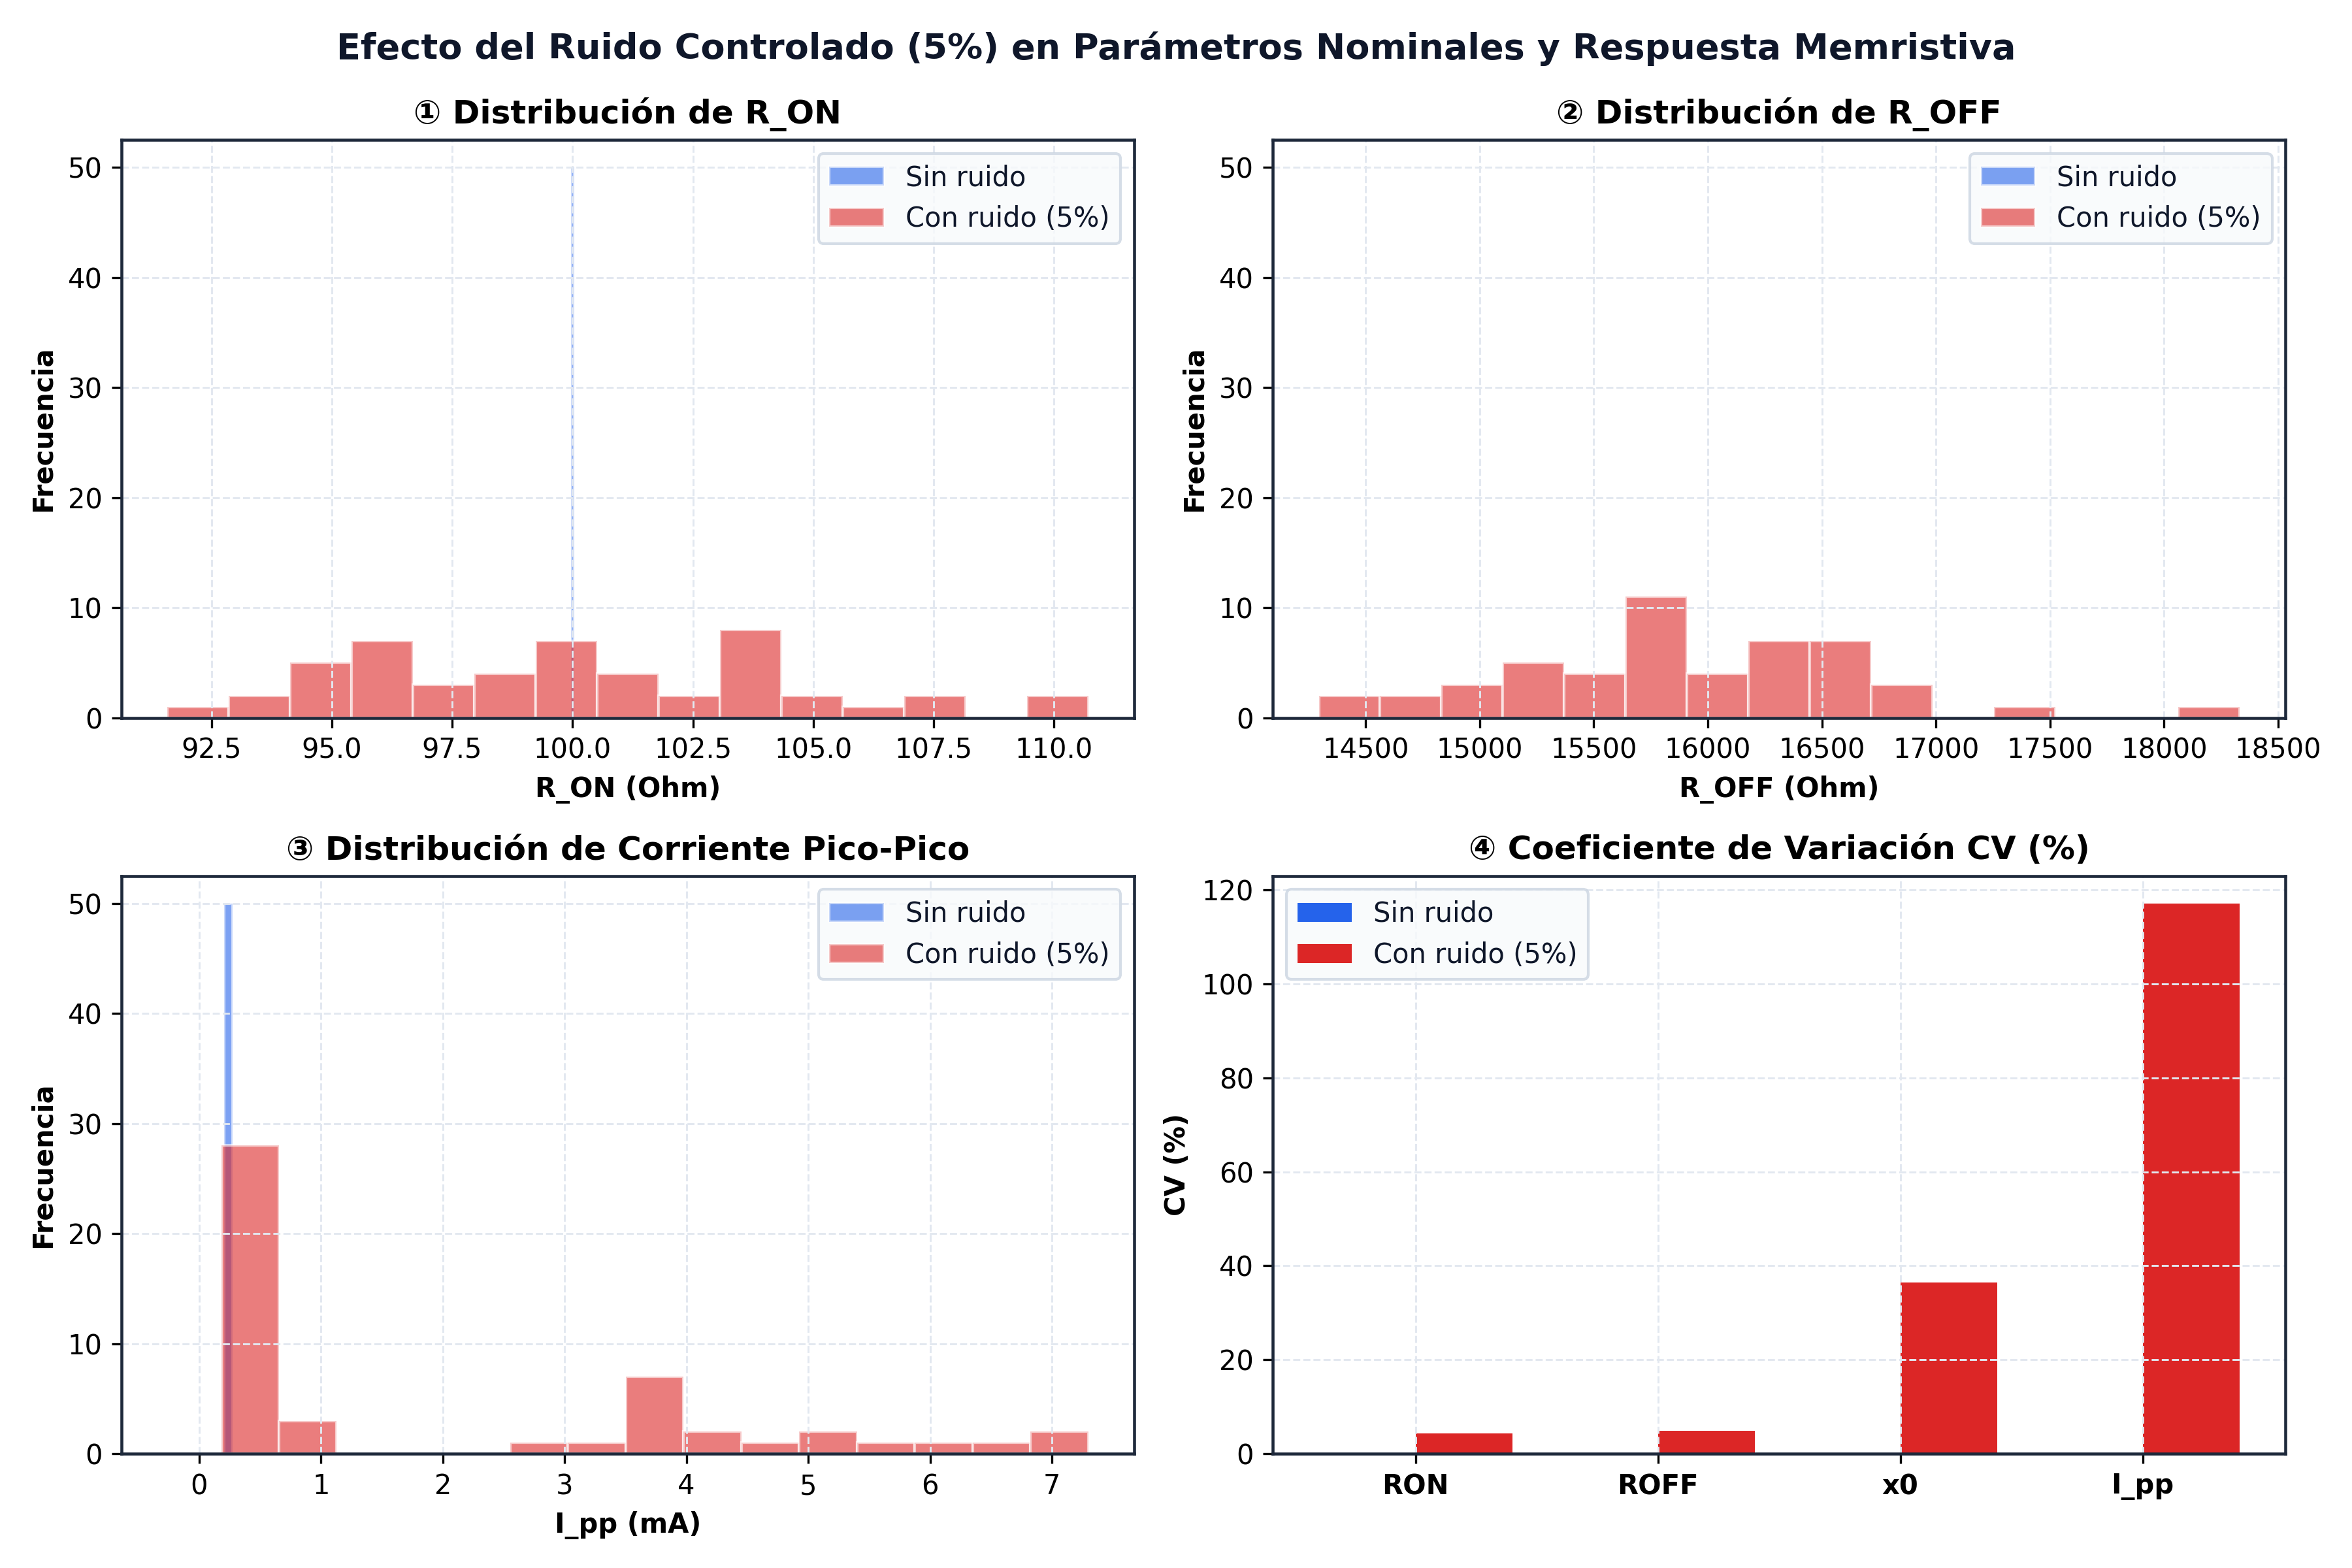
\includegraphics[width=0.7\textwidth]{figuras/fig_11_ruido.png}
    \caption{Sensibilidad del dispositivo a perturbaciones gaussianas del $5\%$ en sus parámetros nominales.}
    \label{fig:11_ruido}
\end{figure}

\textbf{Propósito y Relevancia:} La figura compara las distribuciones de $R_{\mathrm{ON}}$, $R_{\mathrm{OFF}}$ y corriente pico a pico, además del coeficiente de variación, entre dispositivos nominales y dispositivos con perturbaciones paramétricas. No representa una respuesta frecuencial ni permite concluir que el estado del memristor actúe como filtro pasa-bajos.

\begin{figure}[H]
    \centering
    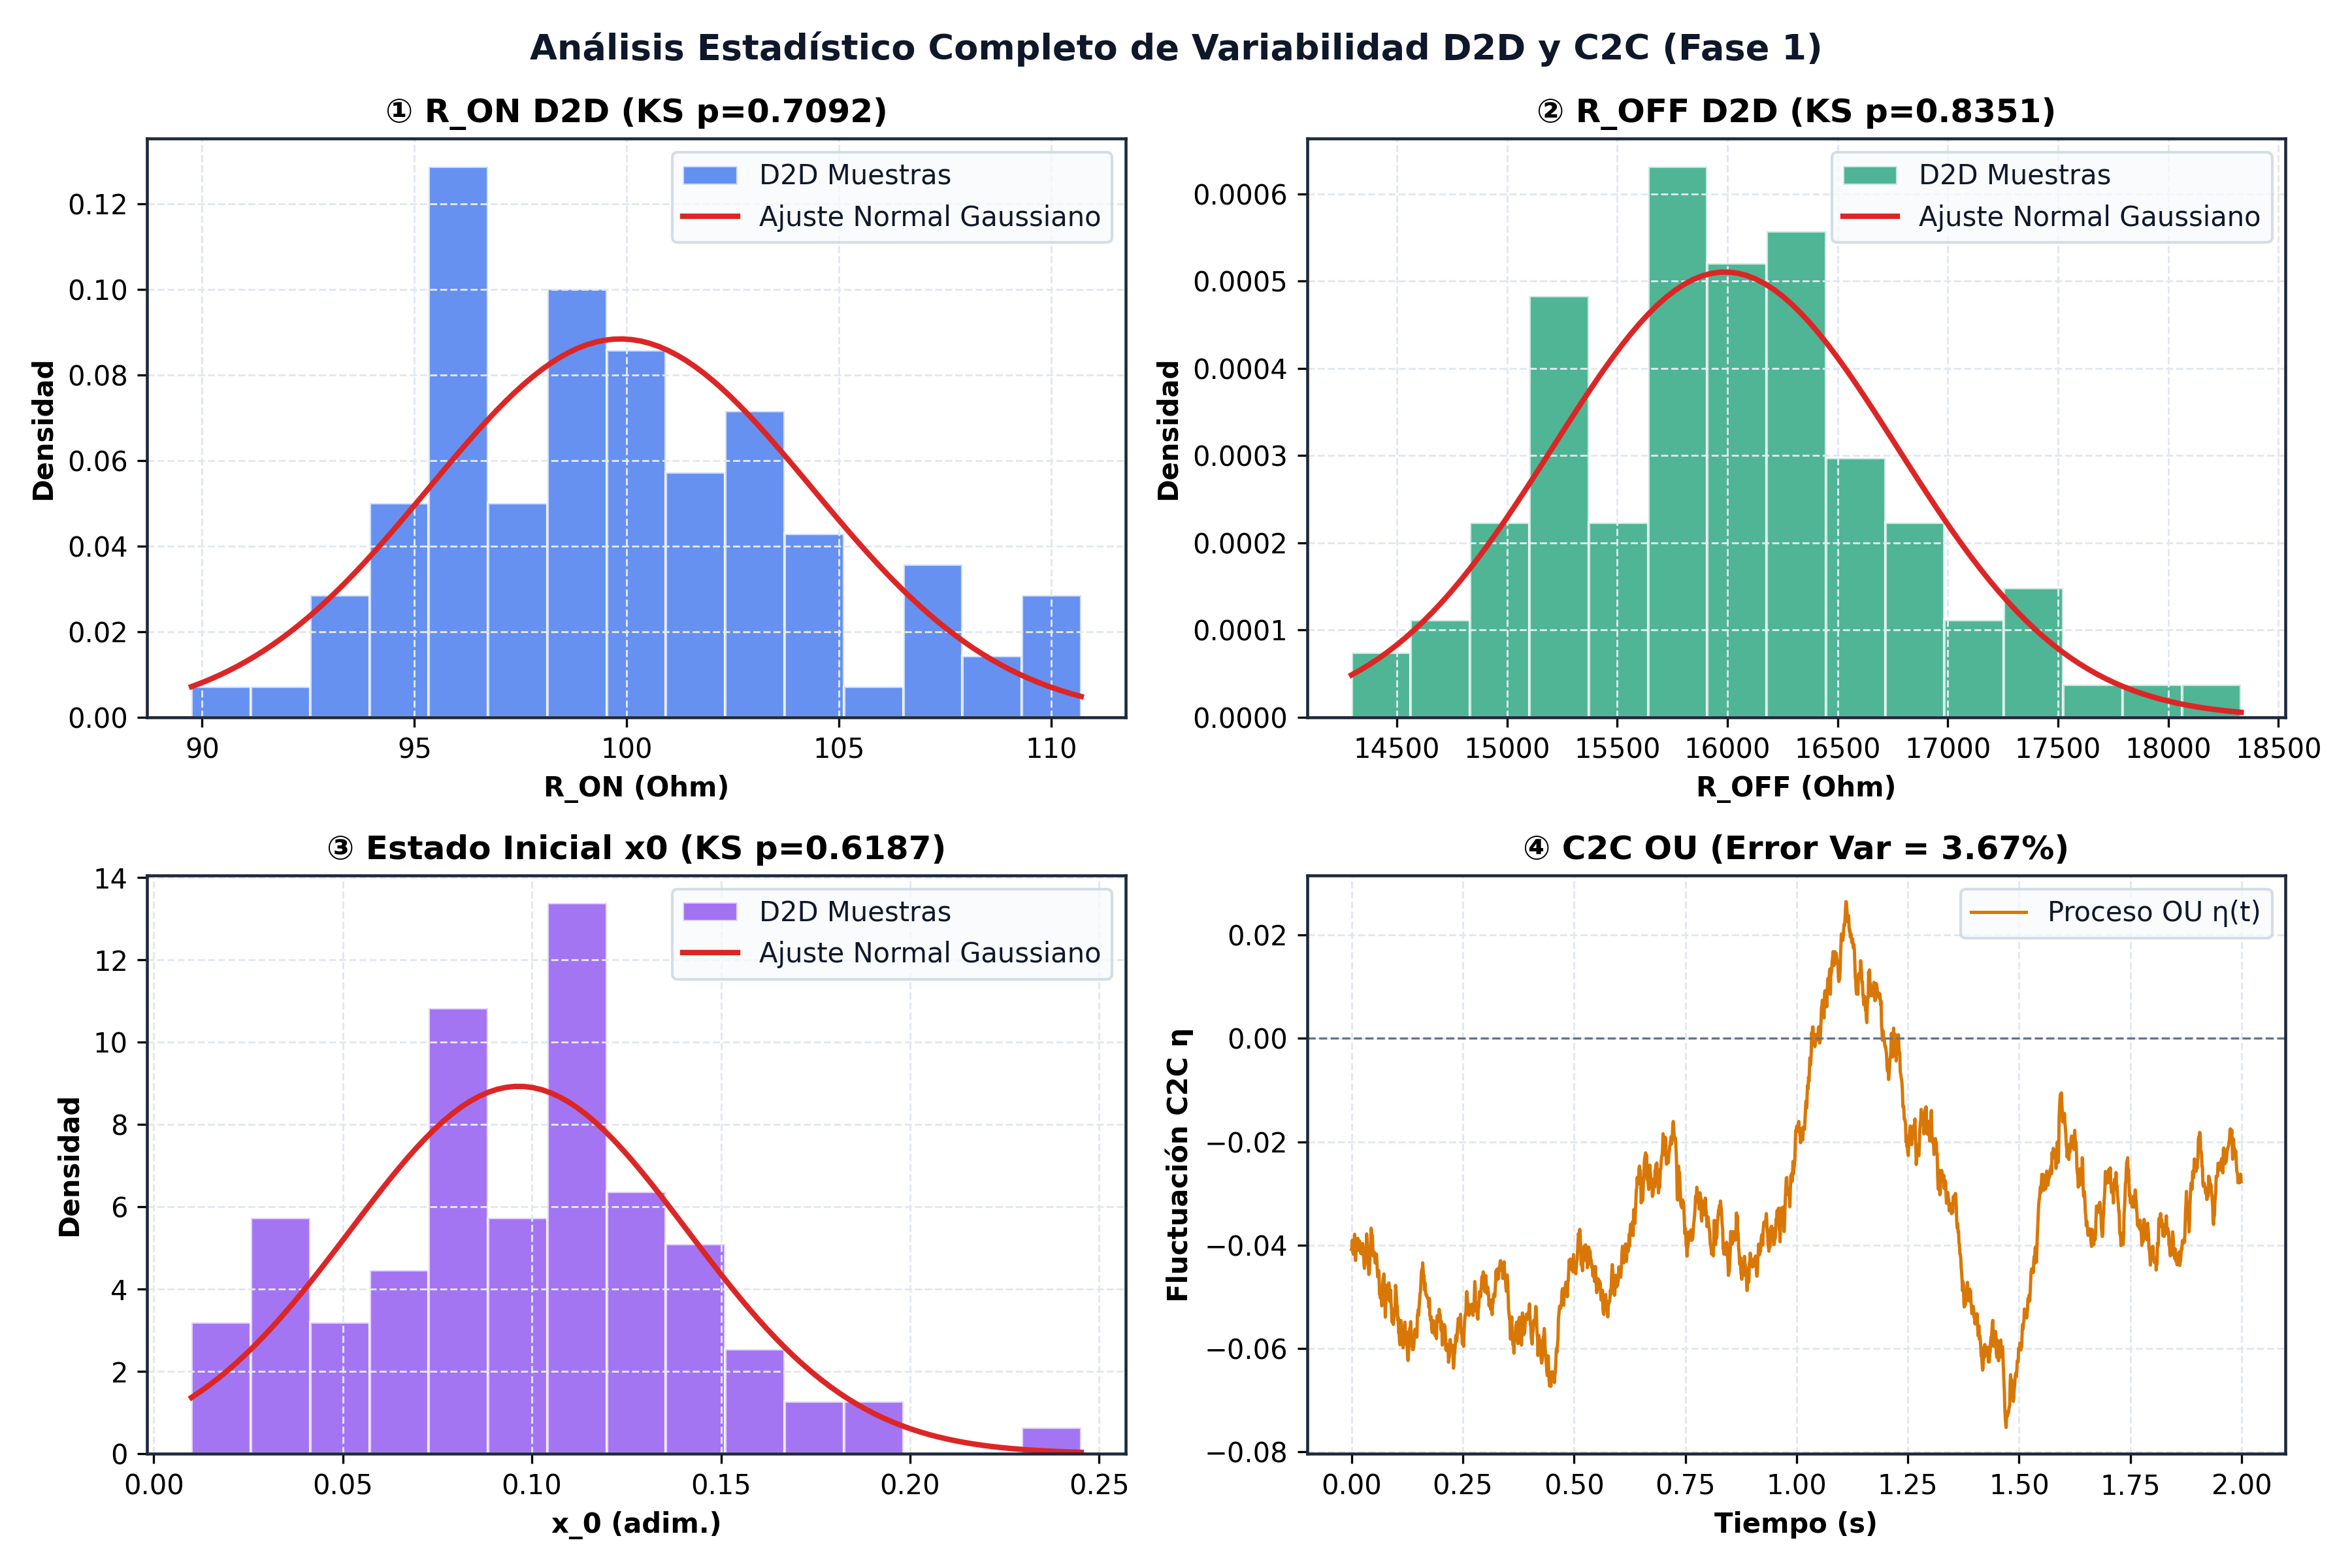
\includegraphics[width=0.8\textwidth]{figuras/fig_12_estadistica.png}
    \caption[Estadística D2D reportada]{Distribuciones D2D y pruebas KS de una corrida archivada distinta del cálculo reproducido con \texttt{05\_d2d\_c2c.py}.}
    \label{fig:12_estadistica}
\end{figure}

Los valores $p$ del panel, incluido $0.7092$ para $R_{\mathrm{ON}}$, proceden de la corrida archivada en \texttt{validacion\_estadistica\_completa.csv}, generada por \texttt{12\_estadistica.py}. Esa rutina usa una muestra distinta y ajusta media y desviación muestrales; no se revalidó la calibración del KS tras estimar esos parámetros con la misma muestra. El valor $0.8959$ informado arriba proviene de \texttt{05\_d2d\_c2c.py}, con los valores nominales para normalizar y contrastar contra $\mathcal{N}(0,1)$. Son análisis diferentes, por lo que sus $p$-valores no son intercambiables; el análisis archivado no se reprodujo en esta revisión.

\textbf{Propósito y Relevancia:} El panel reúne resúmenes estadísticos de muestras simuladas. Estos histogramas describen la población generada por el modelo; no demuestran que esa población reproduzca una distribución experimental ni validan arreglos físicos.
